%% March 2018
%%%%%%%%%%%%%%%%%%%%%%%%%%%%%%%%%%%%%%%%%%%%%%%%%%%%%%%%%%%%%%%%%%%%%%%%%%%%
% AGUJournalTemplate.tex: this template file is for articles formatted with 
% LaTeX
%
% This file includes commands and instructions
% given in the order necessary to produce a final output that will
% satisfy AGU requirements, including customized APA reference formatting.
%
% You may copy this file and give it your
% article name, and enter your text.
%
%%%%%%%%%%%%%%%%%%%%%%%%%%%%%%%%%%%%%%%%%%%%%%%%%%%%%%%%%%%%%%%%%%%%%%%%%%%%
% PLEASE DO NOT USE YOUR OWN MACROS
% DO NOT USE \newcommand, \renewcommand, or \def, etc.
%
% FOR FIGURES, DO NOT USE \psfrag or \subfigure.
% DO NOT USE \psfrag or \subfigure commands.
%%%%%%%%%%%%%%%%%%%%%%%%%%%%%%%%%%%%%%%%%%%%%%%%%%%%%%%%%%%%%%%%%%%%%%%%%%%%
%
% Step 1: Set the \documentclass
%
% There are two options for article format:
%
% PLEASE USE THE DRAFT OPTION TO SUBMIT YOUR PAPERS.
% The draft option produces double spaced output.

%% To submit your paper:
\documentclass[draft,linenumbers]{agujournal2018}
\usepackage{apacite}
\usepackage{graphicx}
\usepackage[demo]{rotating}
% \usepackage{url}    %this package should fix any errors with URLs in refs.
\draftfalse 		% This option makes double space

%%%%%%%
% \usepackage{trackchanges}
% uncomment the line above to use the TrackChanges package to mark revisions 
% if needed.
% The trackchanges package adds five new LaTeX commands:
%
%  \note[editor]{The note}
%  \annote[editor]{Text to annotate}{The note}
%  \add[editor]{Text to add}
%  \remove[editor]{Text to remove}
%  \change[editor]{Text to remove}{Text to add}
%
% complete documentation is here: http://trackchanges.sourceforge.net/
%%%%%%%


% Now, type in the journal name: \journalname{<Journal Name>}

% ie, \journalname{Journal of Geophysical Research}
%% Choose from this list of Journals:
%
% JGR-Atmospheres
% JGR-Biogeosciences
% JGR-Earth Surface
% JGR-Oceans
% JGR-Planets
% JGR-Solid Earth
% JGR-Space Physics
% Global Biochemical Cycles
% Geophysical Research Letters
% Paleoceanography
% Radio Science
% Reviews of Geophysics
% Tectonics
% Space Weather
% Water Resource Research
% Geochemistry, Geophysics, Geosystems
% Journal of Advances in Modeling Earth Systems (JAMES)
% Earth's Future
% Earth and Space Science
% Geohealth
%

\journalname{Water Resource Research}

\begin{document}

%% ------------------------------------------------------------------------ %%
%  Title
% (A title should be specific, informative, and brief. Use
% abbreviations only if they are defined in the abstract. Titles that
% start with general keywords then specific terms are optimized in
% searches)
%% ------------------------------------------------------------------------ %%

% OPTION 1 - Antonio Preziosi
\title{Fine Sediment Deposition and Filtration Under Losing and Gaining Conditions: A Particle-Tracking 
Model Approach}

% OPTION 2 - Antonio Preziosi
% \title{Particle tracking model for kaolinite deposition in flumes under 
% losing or gaining flow conditions}

% OPTION 3 - Antonio Preziosi
% \title{Colloid exchange between a gaining/losing stream and streambed: 
% A particle tracking approach}

% Example: \title{This is a test title}

%% ------------------------------------------------------------------------ %%
%  AUTHORS AND AFFILIATIONS
%% ------------------------------------------------------------------------ %%

% Authors are individuals who have significantly contributed to the
% research and preparation of the article. Group authors are allowed, if
% each author in the group is separately identified in an appendix.)

% List authors by first name or initial followed by last name and
% separated by commas. Use \affil{} to number affiliations, and
% \thanks{} for author notes.
% Additional author notes should be indicated with \thanks{} (for
% example, for current addresses).

% Autores del paper
\authors{Antonio Preziosi-Ribero\affil{1}\thanks{Ciudad Universitaria,
Bogot\'{a}, Colombia}, Aaron I. Packman\affil{2}, Jorge A. Escobar-Vargas\affil{1, 3}, Colin B. Philips\affil{2}, Leonardo David Donado\affil{1}, and Shai Arnon\affil{4}}

% Afiliaciones de los autores
\affiliation{1}{Universidad Nacional de Colombia, Facultad de Ingenier\'{i}a,
Bogot\'{a}, Colombia}
\affiliation{2}{Department of Civil and Environmental Engineering, 
Northwestern University, Evanston, IL, USA}
\affiliation{3}{Departamento de Ingenier\'{i}a Civil, Pontificia Universidad
Javeriana, Bogot\'{a}, Colombia}
\affiliation{4}{Zuckerberg Institute for Water Research, the J. Blaustein Institutes for Deseart Research, Ben-Gurion University of the Negev, Beersheba, Israel}

% \affiliation{4}{Fourth Affiliation}

% \affiliation{=number=}{=Affiliation Address=}
%(repeat as many times as is necessary)

%% Corresponding Author:
% Corresponding author mailing address and e-mail address:

% (include name and email addresses of the corresponding author.  More
% than one corresponding author is allowed in this LaTeX file and for
% publication; but only one corresponding author is allowed in our
% editorial system.)

% Example: \correspondingauthor{First and Last Name}{email@address.edu}

\correspondingauthor{Antonio Preziosi-Ribero}{apreziosir@unal.edu.co}

%% Keypoints, final entry on title page.

% List up to three key points (at least one is required)
% Key Points summarize the main points and conclusions of the article
% Each must be 100 characters or less with no special characters or 
% punctuation

\begin{keypoints}
\item We developed a Particle-Tracking model for fine sediments' deposition taking into account gaining and losing groundwater into the stream
\item Patterns of clay deposition depend on the velocity profile generated by the free surface flow conditions and groundwater vertical flow
\item Fine particle deposition is controlled by gaining or losing groundwater along with the ins-stream processes
\end{keypoints}

% ============================================================================
% ABSTRACT
% ============================================================================

\begin{abstract}
Fine particles' deposition in rivers plays a major role in hyporheic exchange, riverine ecology and biogeochemistry. Indeed, this phenomenon is present in every stream or river at every stage of its flow. However, it is poorly understood in river hydrodynamics and typical continuum models and expressions like the Advection Dispersion Equation have to be modified to represent it accurately. To determine its extent, we developed a numerical Particle-Tracking (PT) model that simulates fine particles' deposition in an idealized sand dune under losing, neutral and gaining groundwater flow conditions. This model takes into account the velocity profiles generated by free surface and groundwater flow and a stochastic function that simulates filtration in a sand bed. We used previous experimental results from a clay deposition experiment in a flume to assess qualitatively how accurate were our simulations. Our results suggest that fine particles' deposition patterns and residence time functions depend heavily on the groundwater flow conditions imposed and bed filtration. Furthermore, the mean behavior of fine particles' deposition is explained by the velocity profiles and filtration inside the bed. However, results also suggest that the deposition is affected by bed heterogeneity and transient effects like changes in permeability and velocity profiles.
\end{abstract}

% ============================================================================
% INTRODUCTION SECTION - NOT CORRECTED FROM PACKMAN'S COMMENTS YET... 02/12 WILL BE DONE
% ============================================================================
\section{Introduction} \label{Introduction}

% 1. GENERALITIES ON SEDIMENT DEPOSITION AND A BRIEF CONCEPT OF WHAT IS CONSIDERED AND HOW DOES IT WORK IN RIVERS (PARTINGTON)
Fine sediment deposition is ubiquitous for all rivers and it is mainly driven by free surface flow conditions \citep{Packman2000,Packman2000b}. Nutrients and pollutants travel through the stream, get deposited in geomorphic controls like dunes, pools or ripples and return to the stream in different places \citep{Buendia2014}. Indeed, these particles travel along streams according to geological and sedimentary conditions. Similarly, this deposition is also dependent on human actions like river restoration \citep{Gartner2012}.

Particles that are named ``fine sediments'' are typically defined as minerals or organic compounds packed in conglomerates with sizes smaller than $10 \ \mu m$ \citep{Drummond2014,Drummond2018}. They are key drivers to processes like nutrient and carbon dynamics and contaminant transport. Moreover, they are well known for deposit in the stream bed, clog it in different spots \citep{Brunke1999} and resuspend to the free flow with some periodicity \citep{Drummond2015} depending on the surface flow driven by extreme events like storms \citep{Drummond2017}. However, their retention in the stream bed is known to affect hyporheic flow, exchange of nutrients and physical properties of the media like porosity and permeability \citep{Crenshaw2002,Mendoza2017}. 

Along with sediment transport, fine particles' deposition has been fostered by land use changes in the latter times \citep{Wohl2015}, and both have effects in the biogeochemical processes as nutrient and carbon cycling \citep{Hope1994,Gottselig2014}, hence, the Hyporheic Exchange (HE). Indeed, fine particle's deposition and transport has effects in the growth of microbial communities and favor denitrification processes due to the lack of oxygen in clogged zones \citep{Navel2011}. Thus, the understanding of fine aprticle dynamics in riverbeds is a challenge for river restoration and management. 

% 3. THE ROAD SO FAR... 
Current literature about HE and sediment deposition includes experiments and observations in laboratory flumes \citep{Elliott1997b,Marion2002,Salehin2004a}. In theses studies recirculating flumes with sand beds are used along with suspended clay in the free stream flow, e.g. Kaolinite, to assess its deposition patterns with different techniques. Nonetheless, only a handful of experiments have evaluated deposition under losing and gaining flow \citep{Fox2014,Fox2018}. 

In the field scale the exchange between surface flows and groundwater has been heavily recorded and modeled at large scale \citep{Woessner2000a,Cardenas2004}. However, these models are focused on passive tracer transport mainly, with some approaches to sediment transport based on the aforementioned flume experiments and assumptions. Moreover, the concentration of fine particles has been quantified in river beds during baseflow and after storm flows to assess deposition and how it is affected by extreme events \citep{Drummond2017}. 


As regards to numerical models, they have mainly focused on estimating hydrodynamic fields and solute transport using the Advection Dispersion Equation (ADE) \citep{Cardenas2006,Cardenas2007f,Cardenas2007b,Boano2007b,BayaniCardenas2008c,Trauth2013}. These models are useful to estimate contaminant transport under different flow conditions, showing that HE changes drastically when taking into account the groundwater flow.  Nonetheless, PT models for estimating deposition under these special conditions are not considered deeply. 

% 4. WHAT IS THE PROPOSED MODEL AND HOW IT WILL SOLVE THIS LACK OF INFORMATION
Therefore, the goal of this study was to implement a numerical particle-tracking model for fine sediments' deposition and filtration that takes into account both, free surface flow and subsurface vertical flow, assuming a losing, neutral or gaining condition for the stream. The set up is inspired in the work by \citet{Fox2014,Fox2018}, and the numerical Particle-Tracking (PT) model is used to estimate fine sediments' deposition patterns using simple rules under the different flow conditions. Our results are compared with the flume experiments to asses how a complex phenomenon like fine particles' deposition is represented by a discretized PT model. 

% ============================================================================
% METHODS SECTION - HOW I'M DOING THAT!
% ============================================================================
\section{Methods} \label{Methods}

\subsection{Conceptual model} \label{Conceptual_Model}

% The conceptual model and how particles move in the domain
Our particle tracking model aims to represent fine sediments' deposition in an idealized sand-bed (figure \ref{Conceptual}). The conceptual model follows the work by \citet{Elliott1997,Elliott1997b,Packman2000,Packman2000a}, and the groundwater conditions are inspired in the experimental setup that has been used by \citet{Fox2014,Fox2018}. Regarding the numerical model, the work by \citet{Li2017} with nutrient transport in rivers is used as a frame for our Particle-Tracking model. In our case, the gaining or losing flux is imposed at the bottom of the domain as a superposition of the velocity field generated by the advective pumping model. The geomorphical and flow conditions for the numerical model are a two dimensional simplification of the experiments performed by previous studies on fine sediments' deposition \citep{Packman2000,Fox2014,Fox2018}(table \ref{TF:Phys_Param}). Moreover, these features are typical of natural sand bed systems \citep{Vanoni1974,Harvey2012,Worman2007,Hunken2007,Mutz2000,Mutz2003}. To generalize the model, non dimensional quantities are used for the comparisons.

% ============================================================================
% Conceptual model of the problem proposed - figure
\begin{figure}[ht]
\centering
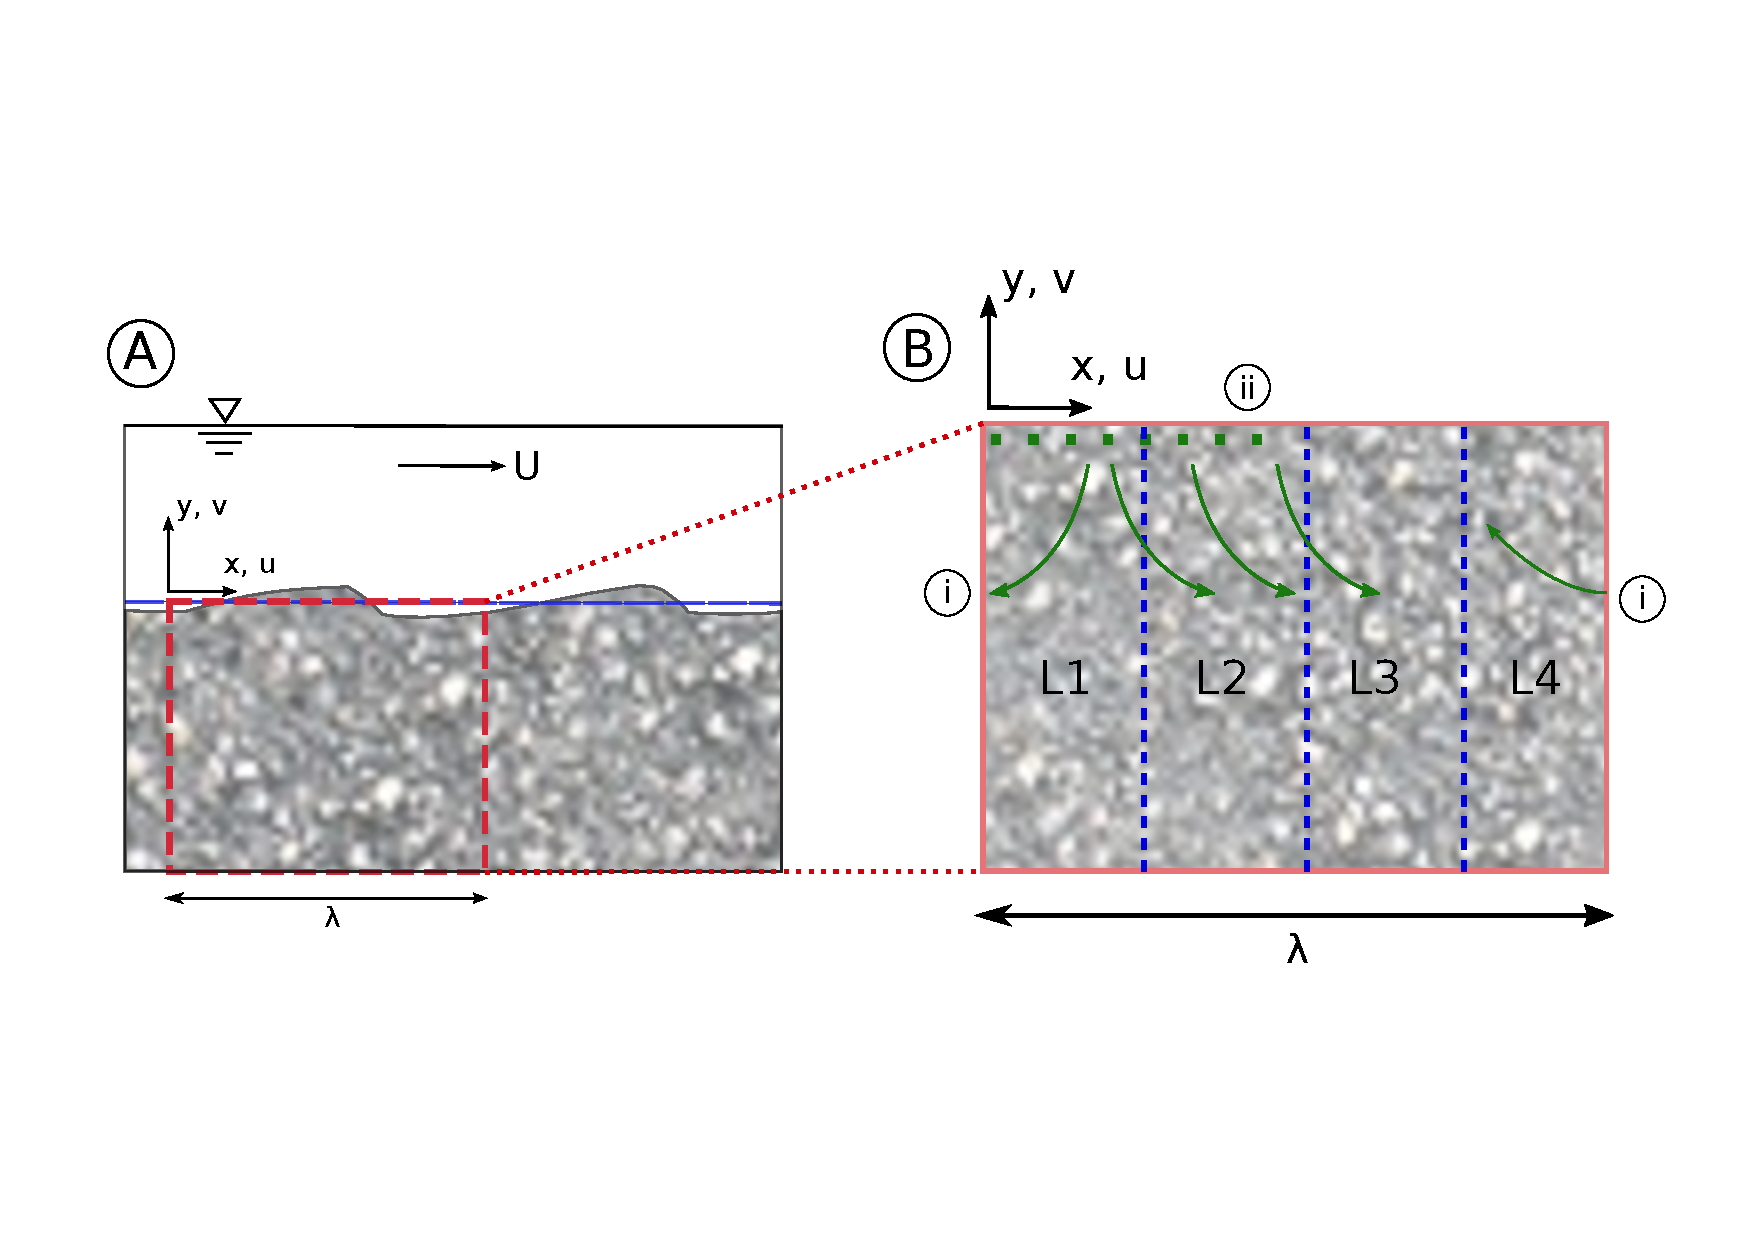
\includegraphics[trim=0.2cm 0.2cm 0.2cm 0.2cm, width=35pc]
{190212_Conceptual.pdf}
\caption{Conceptual model for the posed problem. Panel A: Conceptual model of a typical sand bed with dune shapes. The red box points the model's domain ($\lambda$ is the characteristic dune's wavelength). The blue line shows the mean height of the bed. Panel B: Numerical model's domain. (i) Idealized streamlines from velocity profiles. Note that the lateral boundary conditions of the model are periodic. (ii) Particles are seeded at the top of the domain in the first half of the dune's wavelength and will follow the streamlines and get filtered.}
\label{Conceptual}
\end{figure}
% ============================================================================

% ============================================================================
% TABLE WITH PHYSICAL AND NUMERICAL PARAMETERS FOR THE PARTICLE-TRACKING
% MODEL THAT WAS PROPOSED
% ============================================================================
\begin{table}
\caption{Physical parameters \citep{Packman2000,Fox2014,Fox2018} for the comparison of the Particle-Tracking model implemented.}
\label{TF:Phys_Param}
\centering
\begin{tabular}{l c c}
\hline
PHYSICAL PARAMETERS						    & SYMBOL			& VALUE			\\
\hline
  Flume width $[cm]$  					    & $W$				& 29.0 			\\
  Sediment porosity $[-]$				    & $\theta$			& 0.33 			\\
  Hydraulic conductivity $[cm/s]$ 		    & $K$				& 0.12 			\\
  Flow $[l/min]$						    & $Q$				& 261.0			\\
  Mean stream velocity $[cm/s]$			    & $U$				& 15.0 			\\
  Crossection depth $[cm]$				    & $d_b$				& 20.0 			\\
  Dune wavelegth $[cm]$					    & $\lambda$			& 15.0 			\\
  Water depth $[cm]$					    & $d$				& 8.8 			\\
  Total streambed area $[cm^{2}]$		    & $A$				& 15.1	 		\\
  Imposed GW condition (in/out) $[cm/d]$    & $q_{in}$			& $\pm 12.5$	\\
  Filtering coefficient $[1/cm]$		    & $\lambda_f$		& 0.6			\\
\hline
\end{tabular}
\end{table}
% ============================================================================

The main assumptions of our model are (i) macroscopic processes are considered separately from pore-scale processes, hence the movement of the particles is considered independent from the bed filtration process; (ii) particles do not interact with each other so collision processes are not taken into account; (iii) particles do not change the flow conditions in the media when they are filtered in the bed; and (iv) fine particles' deposition is irreversible.

The computational domain is a box with $\lambda$ side, representing the wavelength of the dune. In the vertical axis, the box has a side $d_b$ that stands for the depth of the sand bed, or the distance between the free surface flow and an impervious layer at the bottom of the domain. The sides of the box are open and they represent a periodic boundary. That is to say that the particles that exit the domain at the right part will re enter at the left side boundary and viceversa (figure \ref{Conceptual}). 

The model's flow conditions are estimated superposing the advective pumping model from previous literature and the groundwater conditions (i.e., losing, neutral or gaining). The particles are seeded in the top part of the domain in the left of the box, that represents the stoss side of the sand dune. Every timestep, particles move according to the velocity field estimated and then the filtration process is estimated using a random number generator. Subsections \ref{Mathematical_model} and \ref{Numerical_model} will explain in depth the moving and trapping/filtering features of the model.

\subsection{Mathematical Model} \label{Mathematical_model}

The velocity fields used for modeling the water flow inside the dune are taken from existing literature \citep{Elliott1997,Packman2000} and groundwater is superposed to them (equations \ref{u} and \ref{v}). The groundwater vertical flow condition is added to the existing profiles (i.e. positive upwards velocity for gaining condition and negative downwards velocity for the losing condition). Here, $x$ and $y$ are the Cartesian coordinates reference axis ($y = 0$ is the top of the domain), $k$ stands for the normalized dune wavelength $(2 \pi / \lambda)$ and $u$ and $v$ for the horizontal and vertical velocity components, respectively. Furthermore, $h_m$ represents the mean pressure over the dune, $K$ stands for the permeability of the media, $d_b$ for the thickness of the bed that is analyzed and $q_{in/out}$ is the component of vertical velocity caused by the groundwater inflow/outflow. 

% Velocity profile equations - From Packman et al. 2000
% use \nonumber if you want to split an equation in different rows and not number a row
\begin{eqnarray}
\label{u}
  u & = & -(kKh_{m}) \cos(kx) [\tanh(kd_b)\sinh(ky) + \cosh(ky)] \\
\label{v}
  v & = & -(kKh_{m}) \sin(kx) [\tanh(kd_b)\cosh(ky) + \sinh(ky)] \pm q_{in/out} 
\end{eqnarray}

All of the quantities are normalized according to the theory developed for flow and transport in sand beds \citep{Elliott1997,Packman2000}. As a result, equations \ref{u} and \ref{v} can be transformed in equations \ref{ustar} and \ref{vstar}. The inflow/outflow velocity $q_{in/out}$ is normalized with the maximum pumping velocity $u_m$. The resulting velocity profiles (figure \ref{Velocities}), exhibit how the addition of the vertical velocity changes the flow direction inside the sand dune and highlights the places where flow recirculation and stagnation are present (figure \ref{Velocities}a and \ref{Velocities}c). The losing flow condition shows that most of the flow is directed downwards (figure \ref{Velocities}A), while the gaining condition shows that flow is going upwards in most of the domain (figurwe \ref{Velocities}c). Moreover, the places where the velocities are close to zero and flowing in opposite directions are shifted by $\pi$ between the two extreme cases modeled (figure \ref{Velocities}a and c). 

% Dimensionless velocity profiles - From Packman with Elliott 
\begin{eqnarray}
\label{ustar}
  u^* & = & -\cos(x^*)[\tanh(d_b^*)\sinh(y^*) + \cosh(y^*)]\\
\label{vstar}
  v^* & = & -\sin(x^*)[\tanh(d_b^*)\cosh(y^*) + \sinh(y^*)] \pm q_{in/out}^*
\end{eqnarray}

% ============================================================================
% Velocity profiles - figure
\begin{figure}[ht]
\centering
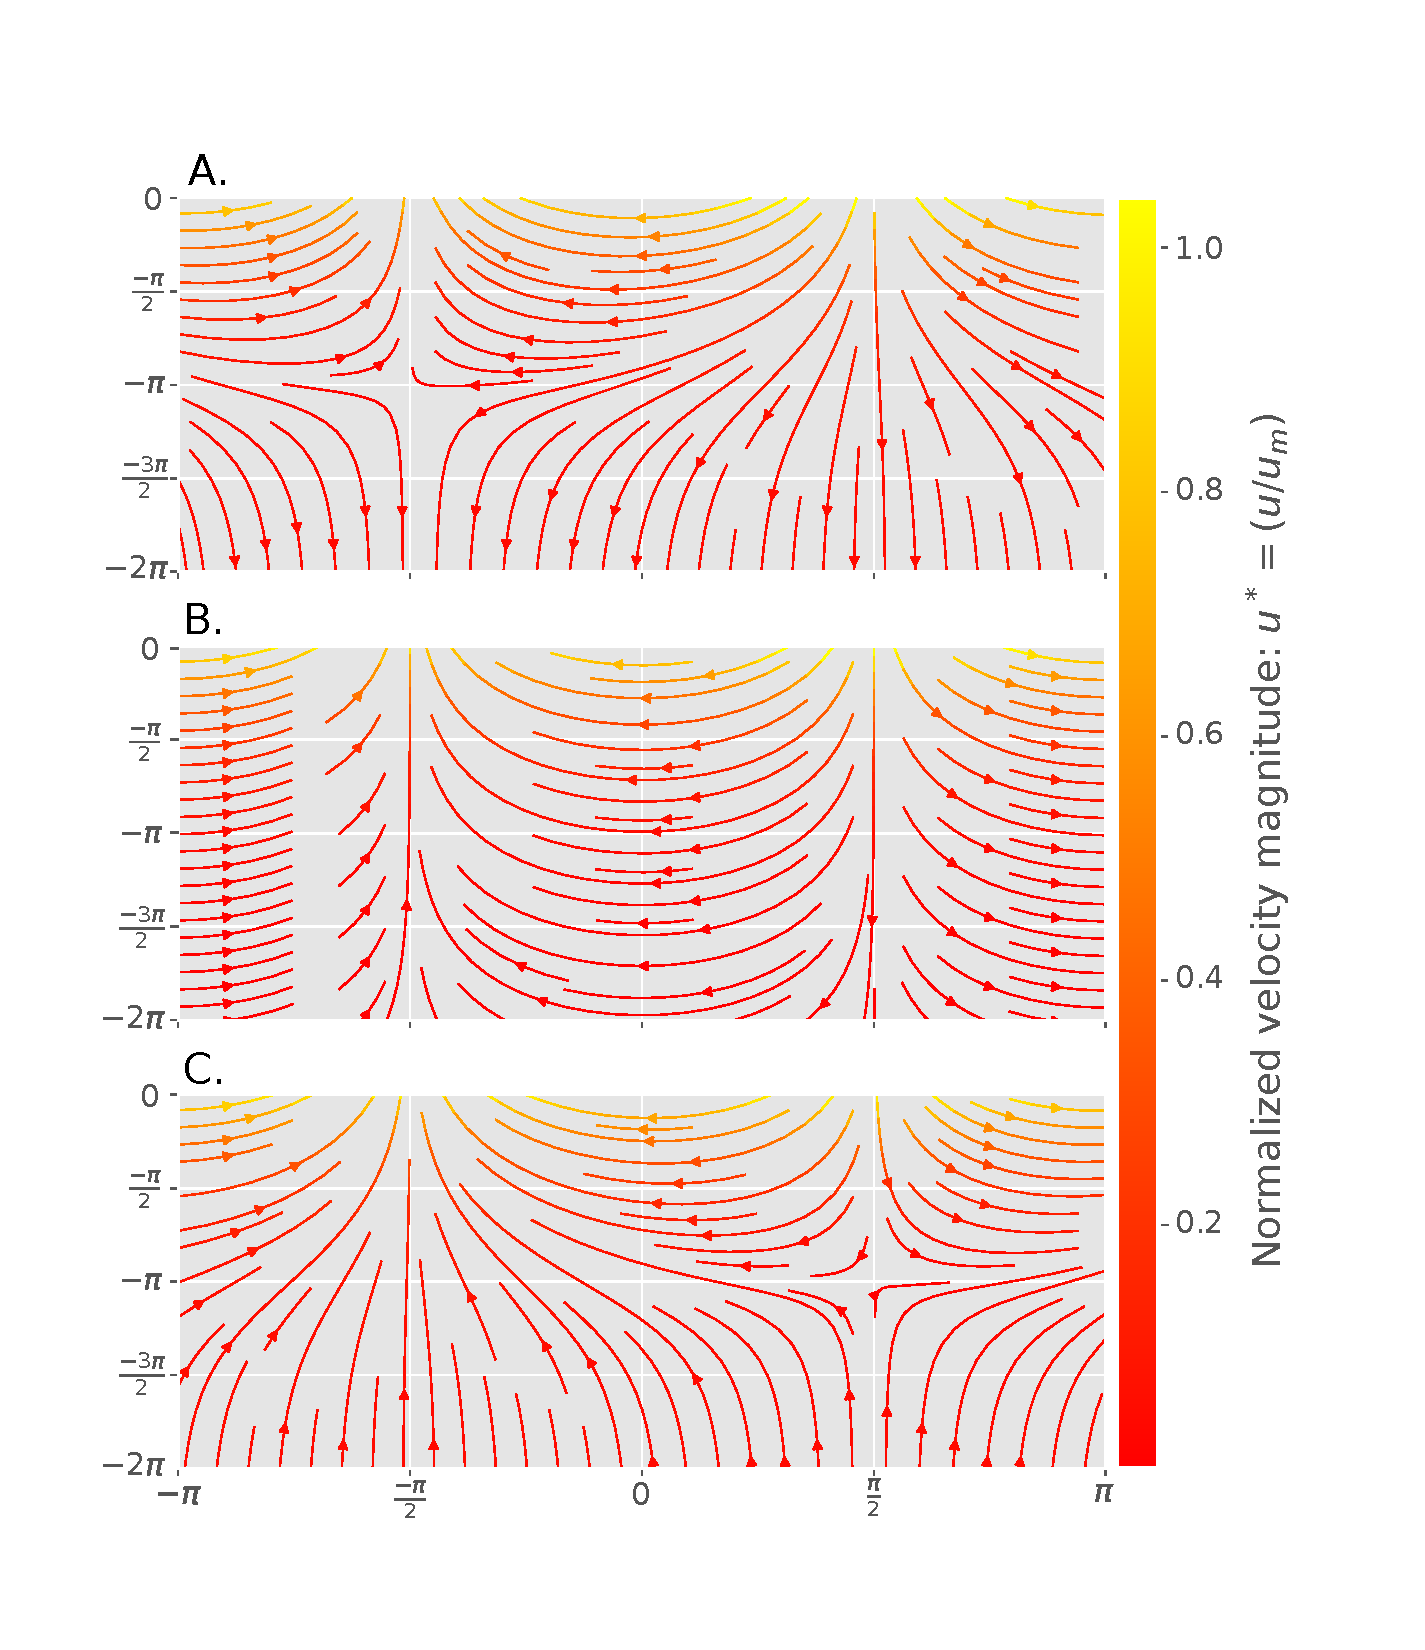
\includegraphics[width=35pc]
{190131_Streamlines.pdf}
\caption{Streamlines plot under different vertical flow conditions: (A) Losing, (B) Neutral and (C) Gaining. Domains are plotted in the interval $[-\pi /2, \pi/2]$ since domain is periodic. The color bar points the magnitude of the velocity vector. Note that the vertical scale is distorted.}
\label{Velocities}
\end{figure}
% ============================================================================

The superposition of the velocity profiles generated with the superposition of the APM and the vertical groundwater flow are physically coherent, since the lowest velocities are present at the bottom of the domain and the highest are located close to the SWI. Moreover, the main dynamics of HE are not suppressed by the gaining/losing conditions imposed by thye vertical groundwater flow.

As regards to the settling velocity, when taking into account a fine particle, e.g. kaoline, with typical density $\rho_p$ \citep{NationalCenterforBiotechnologyInformation}, mean diameter $d_p$ \citep{Fox2014}; and taking $u_0$ as the mean velocity in the subsurface (which is taken to be greater than the maximum obtained from equations \ref{u} and \ref{v}), $\mu_f$ as water's dynamic viscosity \citep{Cengel2006}, and $l_0$ as the characteristic length of the phenomenon which is similar to the dune height \citep{Fox2018}; the value of the stokes number is less than 1.0, i.e. a given kaolinite particle will follow the streamlines of the velocity profile without diverging from them \citep{Tropea2007} (equation \ref{STK}).

% Stokes number calculation
\begin{equation}
 \label{STK}
 	Stk = \frac{\rho_p d_p^2 u_0}{18 \mu_f l_0} = \frac{2650 \frac{kg}{m^3} \cdot [384 \times 10^{-6}m]^2 \cdot 0.01 \frac{m}{s}}{18 \cdot 1.519 \times 10^{-3}Pa \ s \cdot 0.01 m} = 0.014
 \end{equation}

The modeled clay particles follow the streamlines formed by the velocity profiles described in equations \ref{ustar} and \ref{vstar}. The mathematical model starts with the transport of particles along given streamlines, i.e. the Advection Dispersion Equation (ADE) (equation \ref{ADE}). Here, $C$ stands for the concentration of the particles, $u$ and $v$ for the horizontal and vertical velocities, respectively; $D$ for the mechanical dispersion coefficient and $S$ for rate of particles removal due to filtration \citep{Packman1997}.

% Advection Dispersion Equation with just advection!!!!
\begin{equation}
 \label{ADE}
 	\frac{\partial C}{\partial t} \ + u \frac{\partial C}{\partial x} \ + \ v \frac{\partial C}{\partial y} \ = \ D \bigg(\frac{\partial^2 C}{\partial x^2} + \frac{\partial^2 C}{\partial y^2}\bigg) - S
\end{equation}

The dispersion process can be neglected in particle transport in porous media \citep{Mau1992}, so the ADE can be transformed into an equation that represent a filtration process over a given velocity field (equation \ref{ADE2}). Here, the material derivative of concentration equals the rate of removal of particles over time.

\begin{equation}
 \label{ADE2}
 	\frac{D C}{D t} \ = \frac{\partial C}{\partial t} \ + \ u \frac{\partial C}{\partial x} \ + \ v \frac{\partial C}{\partial y} \ = \ - S
\end{equation}

The rate of particles' removal $S$ can be expressed with the aid of the filtration coefficient $\lambda_f$, the seepage velocity $U = \partial s / \partial t$ (where $s$ is the path traveled by the particle), and the concentration $C$ of the analyzed particles as follows:

\begin{equation}
 \label{lambdaf}
 	S = \lambda_f \frac{\partial s}{\partial t}C
\end{equation}

When replacing the value of $S$ of equation \ref{lambdaf} in equation  \ref{ADE2}, the expression for particles' filtering becomes: 

\begin{equation}
 \label{filtration}
 	\frac{\partial C}{\partial s} = -\lambda_f C
\end{equation}

This model is consistent with previous models of colloidal transport in porous media \citep{Domenico1998}. The key outcome of the mathematical model is that a filtration process along steady streamlines can be expressed as a first order reaction. 

\subsection{Numerical Model} \label{Numerical_model}

The numerical model proposed is similar to the one used by \citet{Packman2000}. Its logical process is divided in three parts that use the discrete versions of equations \ref{ADE2} and \ref{filtration}. The first step calculates the displacement of particles using $\bar{x}(t + \Delta t) = x(t)  + u \cdot \Delta t$ \citep{Li2017}. Hence, each timestep the model takes into account the previous position of each particle and uses the velocity fields to determine its velocity at the point where it is. 

After estimating each particle's position, the filtration process over the timestep is estimated calculating the probability $p$ that the particle stops inside the domain \citep{Prickett1981}:

% Simplification of the continuum - from eulerian to particles
\begin{equation}
\label{Filt_disc}
	p = 1 - e^{-\lambda_f \Delta s} \approx \lambda_{f} \Delta s
\end{equation}

This assumption holds since the size of the timestep $\Delta t$ is small enough to ensure the validity of the Taylor's expansion \citep{Li2017}.

The end of every timestep consists of counting the amount of particles that are still in the domain, which is divided in filtered particles that will remain still for the rest of the simulation; and moving particles, which have not been filtered yet. Besides, the model accounts for the particles that went out of the domain at the top boundary. Those particles are counted as escaped particles and they don't come back to the domain again during the simulation.

The boundary conditions at the right and left walls of the model are periodic. Namely, the streamlines in the left and right boundaries of the domain are connected and particles will cross the left boundary and appear at the right part of the domain and viceversa. Regarding the bottom boundary, ṕarticles are not allowed to cress it. On the other hand, any particle whose $y^* > 0$ is counted as an escaped particle, as mentioned before. 

The particle-tracking simulations were performed under similar conditions to the ones proposed in table \ref{TF:Phys_Param}. The cases were modeled with $2x10^5$ particles for each vertical flow condition imposed (Losing, Neutral and Gaining). The total simulation time ensured that all of the seeded particles were filtered or escaped the domain by the end of the simulation. As regards to the initial condition, the particles are seeded evenly distributed at the top of the domain and just in the left portion of it ($0 < x^* < \pi$), since particles seeded at the right part of the domain ($\pi < x^* < 2\pi$) will immediately escape due to the velocity profiles provided for the particle flow, as shown in figure \ref{Velocities}. 

% About the relative concentration windows where the results are analyzed.
Each simulation's results are then grouped to get information to be compared with experiments \citep{Fox2014,Fox2018}. For that purpose, the model's domain is superposed with a mesh of $100 x167$ squares with $\pi / 50$ size. For every timestep, the number of particles in each square is counted to generate concentration maps. The size of the squares was selected visually, ensuring that results were representative for every one of the three modeled cases. It is worth mentioning that the mesh used for counting particles has no relationship with the computational PT simulation and it is just used to count particles \citep{Xue2017}.

% ============================================================================
% RESULTS SECTION
% ============================================================================
\section{Results}  \label{Results}

% 0. VELOCITY PROFILES UNDER DIFFERENT CONDITIONS WHEN SOLVING FOR THE DIFFERENT IN/OUT VALUES
The velocity profiles that result from equations \ref{ustar} and \ref{vstar} (figure \ref{Velocities}) show substantial differences among them. Indeed, there is a preferential flow going upwards or downwards if the imposed condition is a gaining or losing flow, respectively. Furthermore, there is a no flow zone in the losing and gaining conditions formed by the addition of a vertical flow to a neutral flow condition. Consequently, there is a recirculation zone in the losing and gaining cases, though they are in different places according to the case. Namely, in the gaining condition it is located in the right part of the domain, while for the losing condition it is located at the left. Moreover, the results obtained in the velocity profiles are observed in the experiments ran by \citet{Fox2018}.

Furthermore, the maximum velocity in each profile is located in a different place. In particular, in the losing condition the maximum velocity is in the negative direction at the stoss side of the domain, while in the gaining case it is located in dune's lee. However, for the neutral condition the maximum velocity is located in two parts of the domain but pointing in a different direction; one located in the stoss and the second in the lee. Despite the fact that particles follow the streamlines of the velocity profiles, their deposition is not uniform because of their inflow position at the bed surface (dune's stoss side), and because of the filtering process along the streamlines.

% ============================================================================
% Logarithm of concentration - figure
\begin{sidewaysfigure}
\centering
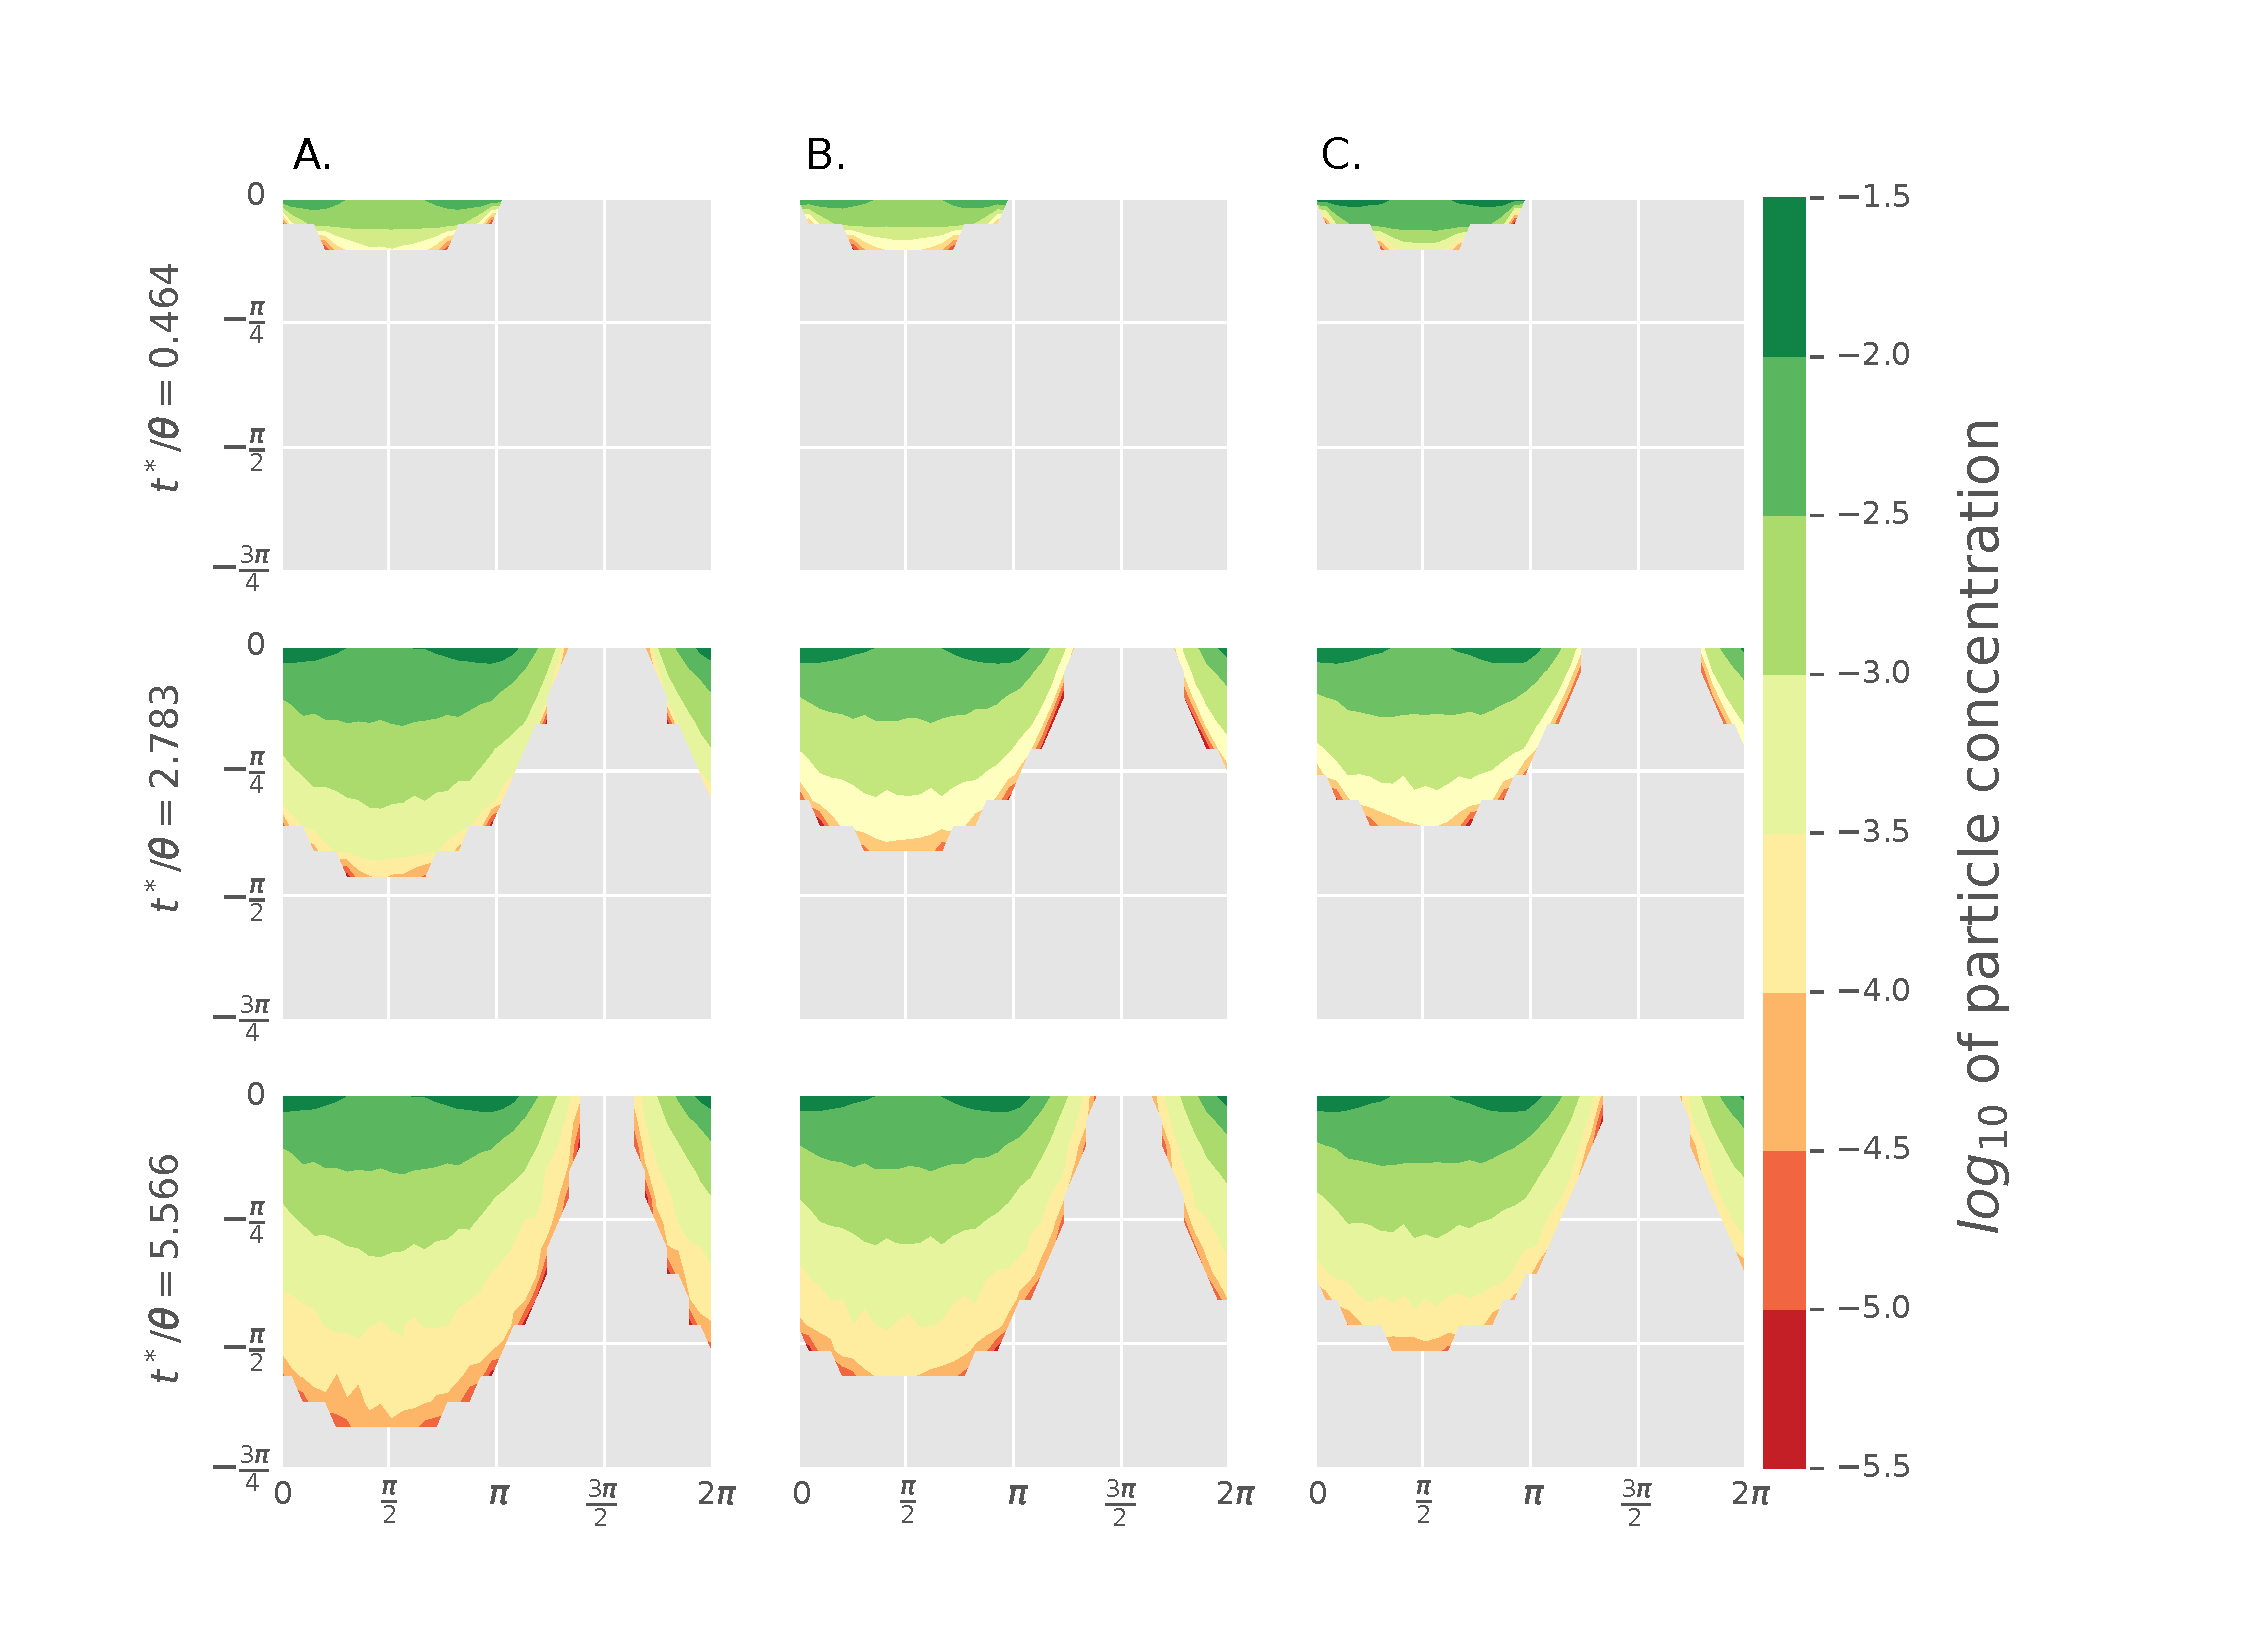
\includegraphics[trim=0.2cm 0.2cm 0.2cm 0.2cm, width=60pc]
{190131_Logplot.pdf}
\caption{Logarithm of total number of particles deposited for different times (rows), and under different inflow/outflow conditions (columns). (A) Losing condition, (B) Neutral condition and (C) Gaining condition (Note that axis are not to scale).}
\label{Logmap}
\end{sidewaysfigure}
% ============================================================================

Both, horizontal and vertical extents of the particle deposition are dependent on the velocity profiles, hence the vertical flow conditions that are imposed to the numerical model. On one hand, the overall behavior of the streamlines for the gaining condition tend to circulate faster inside the sand bed domain and go out to the top boundary faster than in the losing condition. On the other hand, the neutral condition shows definite streamlines that are perfectly layered (figure \ref{Velocities}).

Fine particles' deposition pattern is similar for early times, though their internal distribution is different between the analyzed cases (figure's \ref{Logmap} first row). The maximum depth reached by the particles' front and their shape are the same. However, the internal distribution of particles is different, i.e. in the gaining condition the distribution of particles in the top part of the domain filled by them is more evenly distributed than in the neutral and losing cases. 

In addition, for later times a particular feature arises near the last quarter of the domain, where a gap is formed and no particles are present even at the top of the domain. This position marks the place where particles go out of the domain. Nevertheless, this gap is different for the three modeled conditions; in the losing case it is narrower than in the neutral and gaining ones. The difference between these gaps that arise from the deposition of particles at the right part of the domain is clearly influenced by the shape of the streamlines (figure \ref{Velocities}).

A perceptible difference between particles' deposition can be spotted when analyzing the width the gap formed between the places where particles are deposited. This result is clearly linked to the shape of the velocity profiles and marks the place where particles that are recirculated go out of the domain to the free stream flow. This gap is different in size according to the conditions that are being modeled (figure \ref{Logmap}). Namely, for the losing condition the gap is narrow, and it tend to stretch in neutral and gaining conditions. The particles that are deposited at the right part of the domain come from the streamlines that cross the left boundary of the domain and continue to the left part. 

% 2. BEHAVIOR OF PARTICLES' IN TIME - HOW THEY GET DEPOSITED AND recirculated IN TIME ACCORDING TO THE FLOW CONDITIONS
Besides analyzing particles' in space, we can assess their behavior over time with the results of our model (figure \ref{Pvst}). The relative number of particles that are moving inside the domain (figure \ref{Pvst} blue line), filtered (figure \ref{Pvst} purple line) and particles that have escaped over the top boundary (figure \ref{Pvst} red line). In particular, even with identical filtering coefficients, the amount of particles that remain in the domain and that are recirculated varies significantly betwixt vertical flow conditions imposed. In the gaining case (figure \ref{Pvst}c) the number of particles that remain inside the domain is less than in the neutral (figure \ref{Pvst}b) and losing cases (figure \ref{Pvst}a). Put differently, the number of particles that escape the domain at the top boundary is proportional to the vertical groundwater flow imposed.

% ============================================================================
% Particles in time - figure
\begin{sidewaysfigure}
\centering
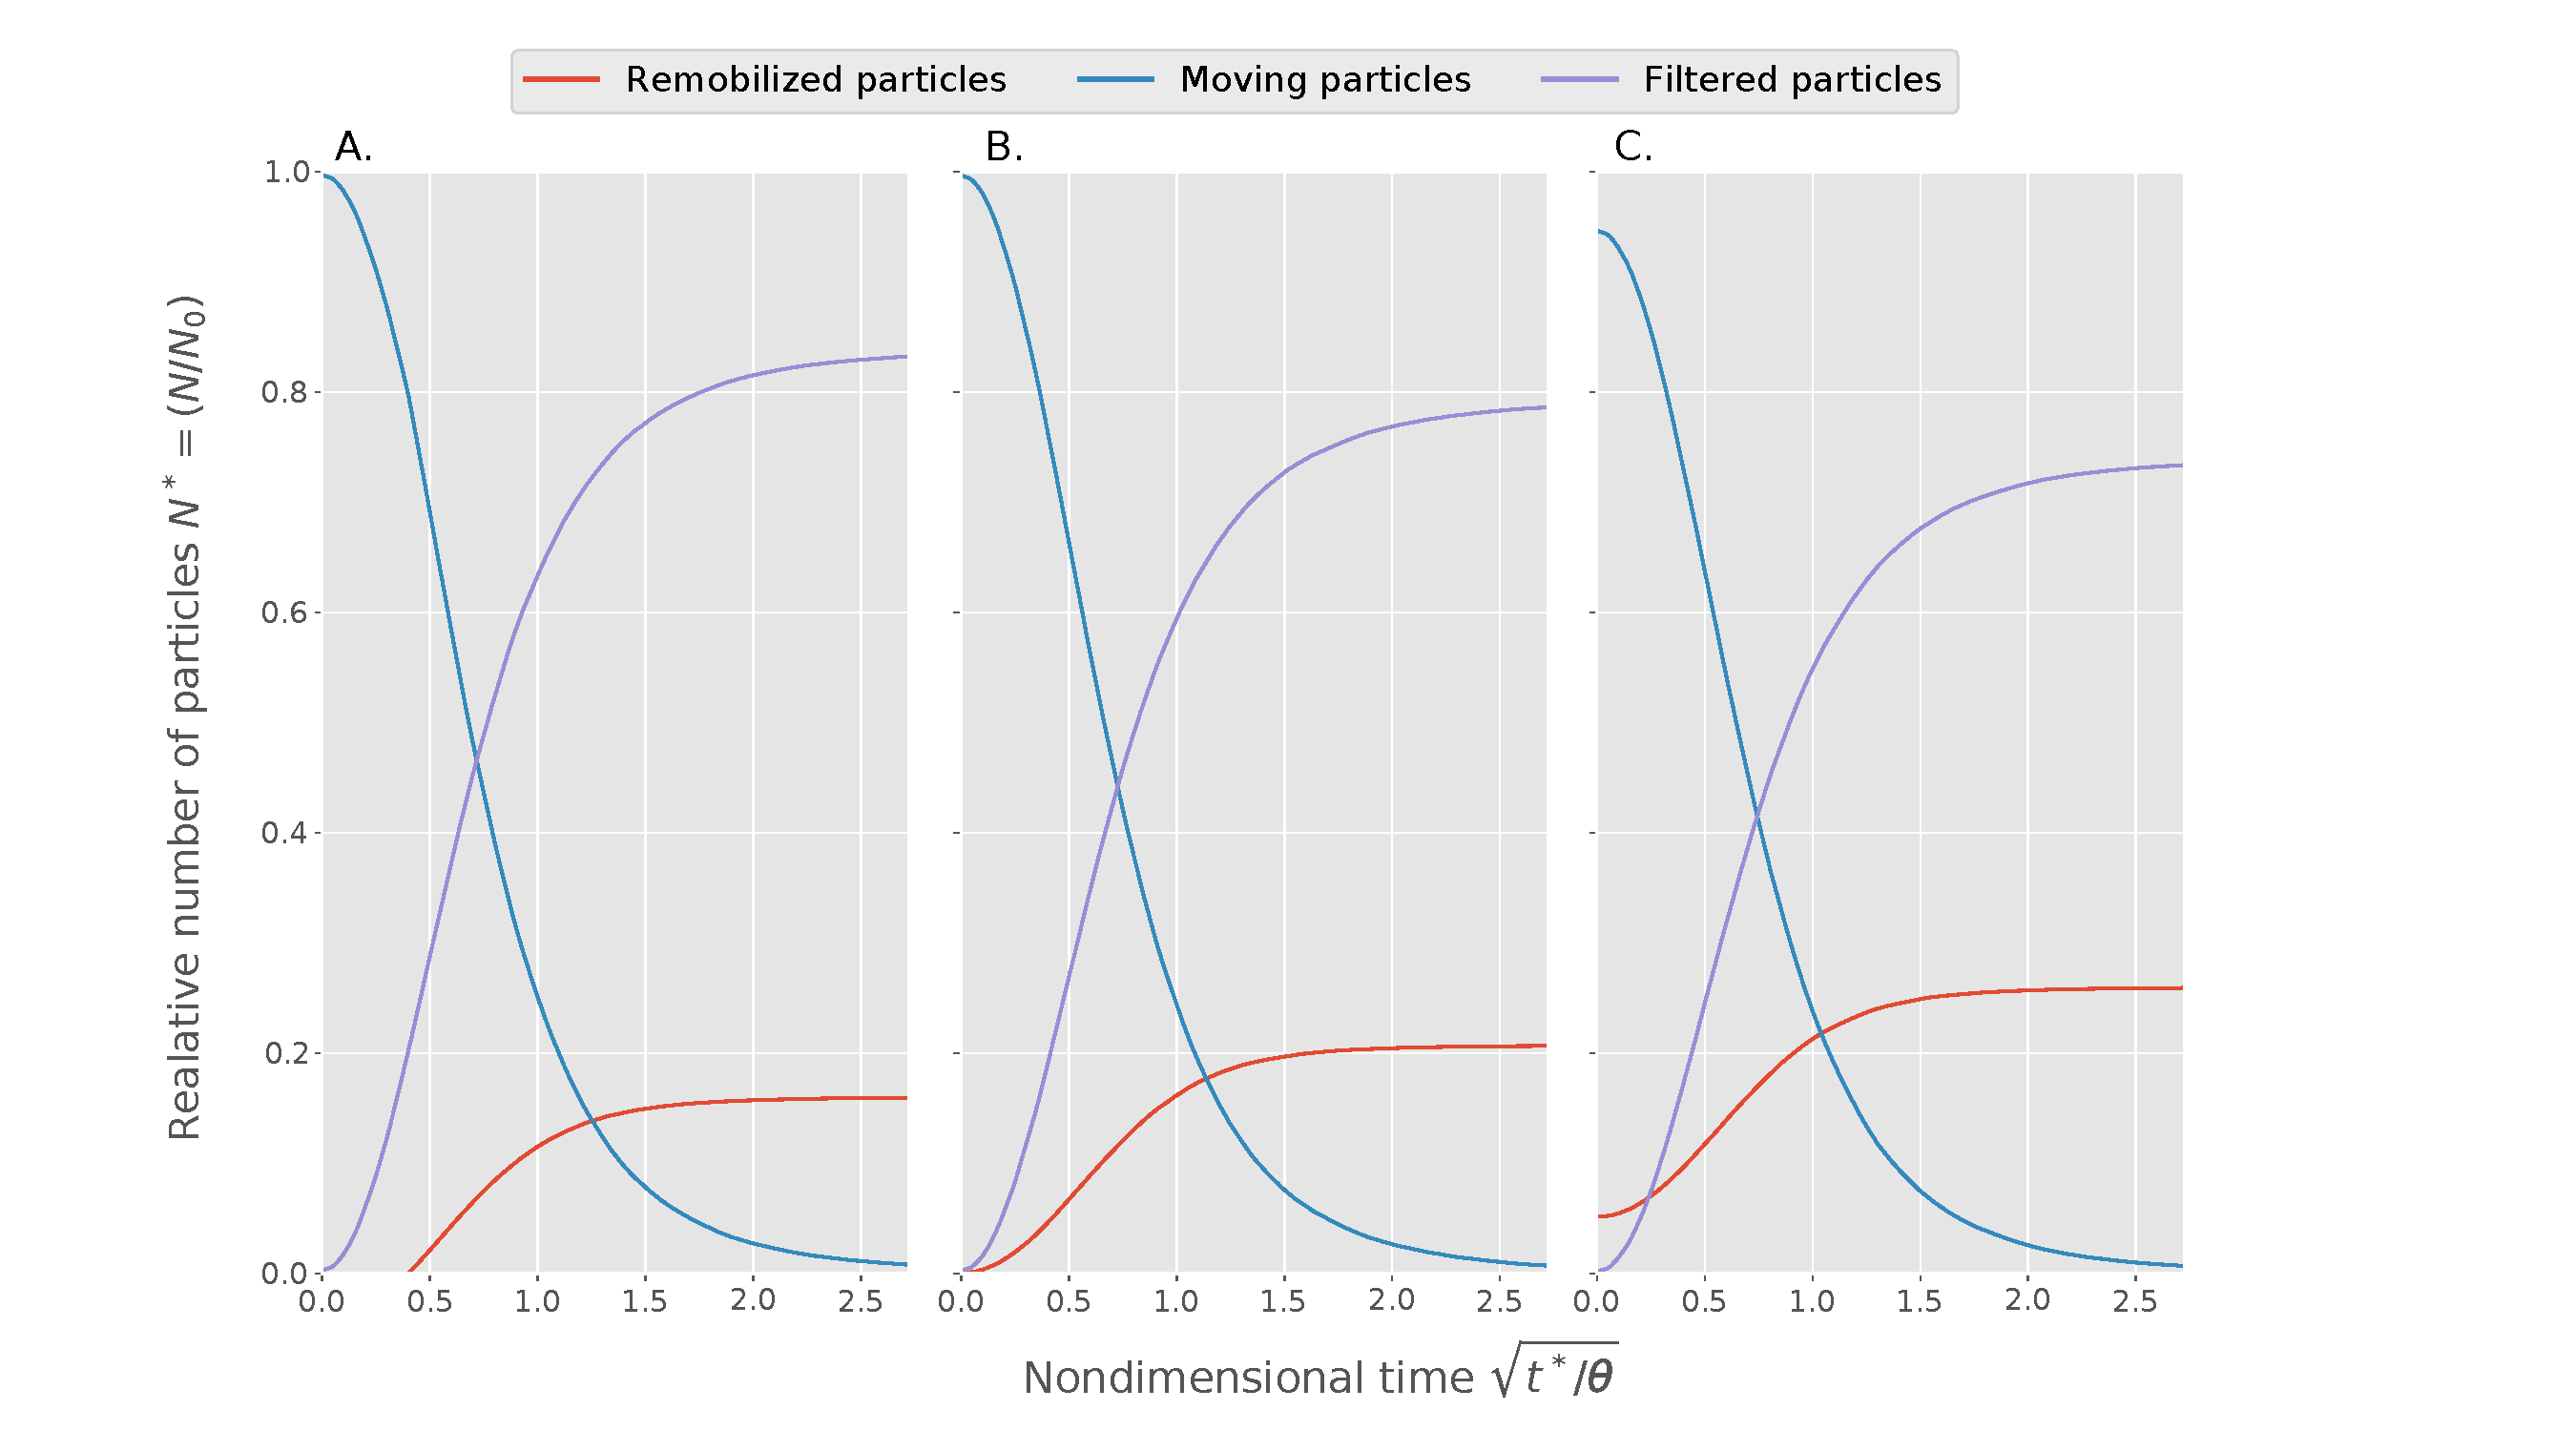
\includegraphics[trim=0.2cm 0.2cm 0.2cm 0.2cm, width=60pc]
{190131_Pvst.pdf}
\caption{Particle's behavior over time. (A) Losing condition. (B) Neutral condition and (C) Gaining condition.}
\label{Pvst}
\end{sidewaysfigure}
% ============================================================================

The expected ensemble continuum behavior of fine particles' deposition is recovered by our PT model. Namely, the filtration process is expected to remove particles in an exponential way and the model is representing this phenomenon. Indeed, this decrease corresponds to the exponential decrease that results from solving equation \ref{Filt_disc} in a typical filtration problem. Furthermore, the presence of particles inside the domain is determined by the filtration coefficient and the imposed vertical groundwater flow.  

% 4. RESIDENCE TIME AND PORTION OF PARTICLES INSIDE THE DOMAIN AT ANY GIVEN TIME.
Besides particles' location in space and time, the PT model can estimate the Residence Time Function (RTF). This feature points the fraction of mass that entered the bed in a time near $t = 0$ and is present inside the domain after a given time $\tau$ \citep{Elliott1997,Packman2000}. For small times $\tau$ close to zero, the value of the RTF is $1.0$, and as $\tau$ increases some of the particles would have escaped the domain. Since the RTF is normalized by the total number of particles (figure \ref{RTF}), the resulting curve is interpreted as the cumulative distribution function (CDF) of particles inside the domain. Moreover, since the filtration process is non reversible, the RTF will never be equal to zero, or put differently, the particles will not be flushed out of the domain unless there is no filtration.

% ============================================================================
% Residence time function - figure
\begin{figure}[ht]
\centering
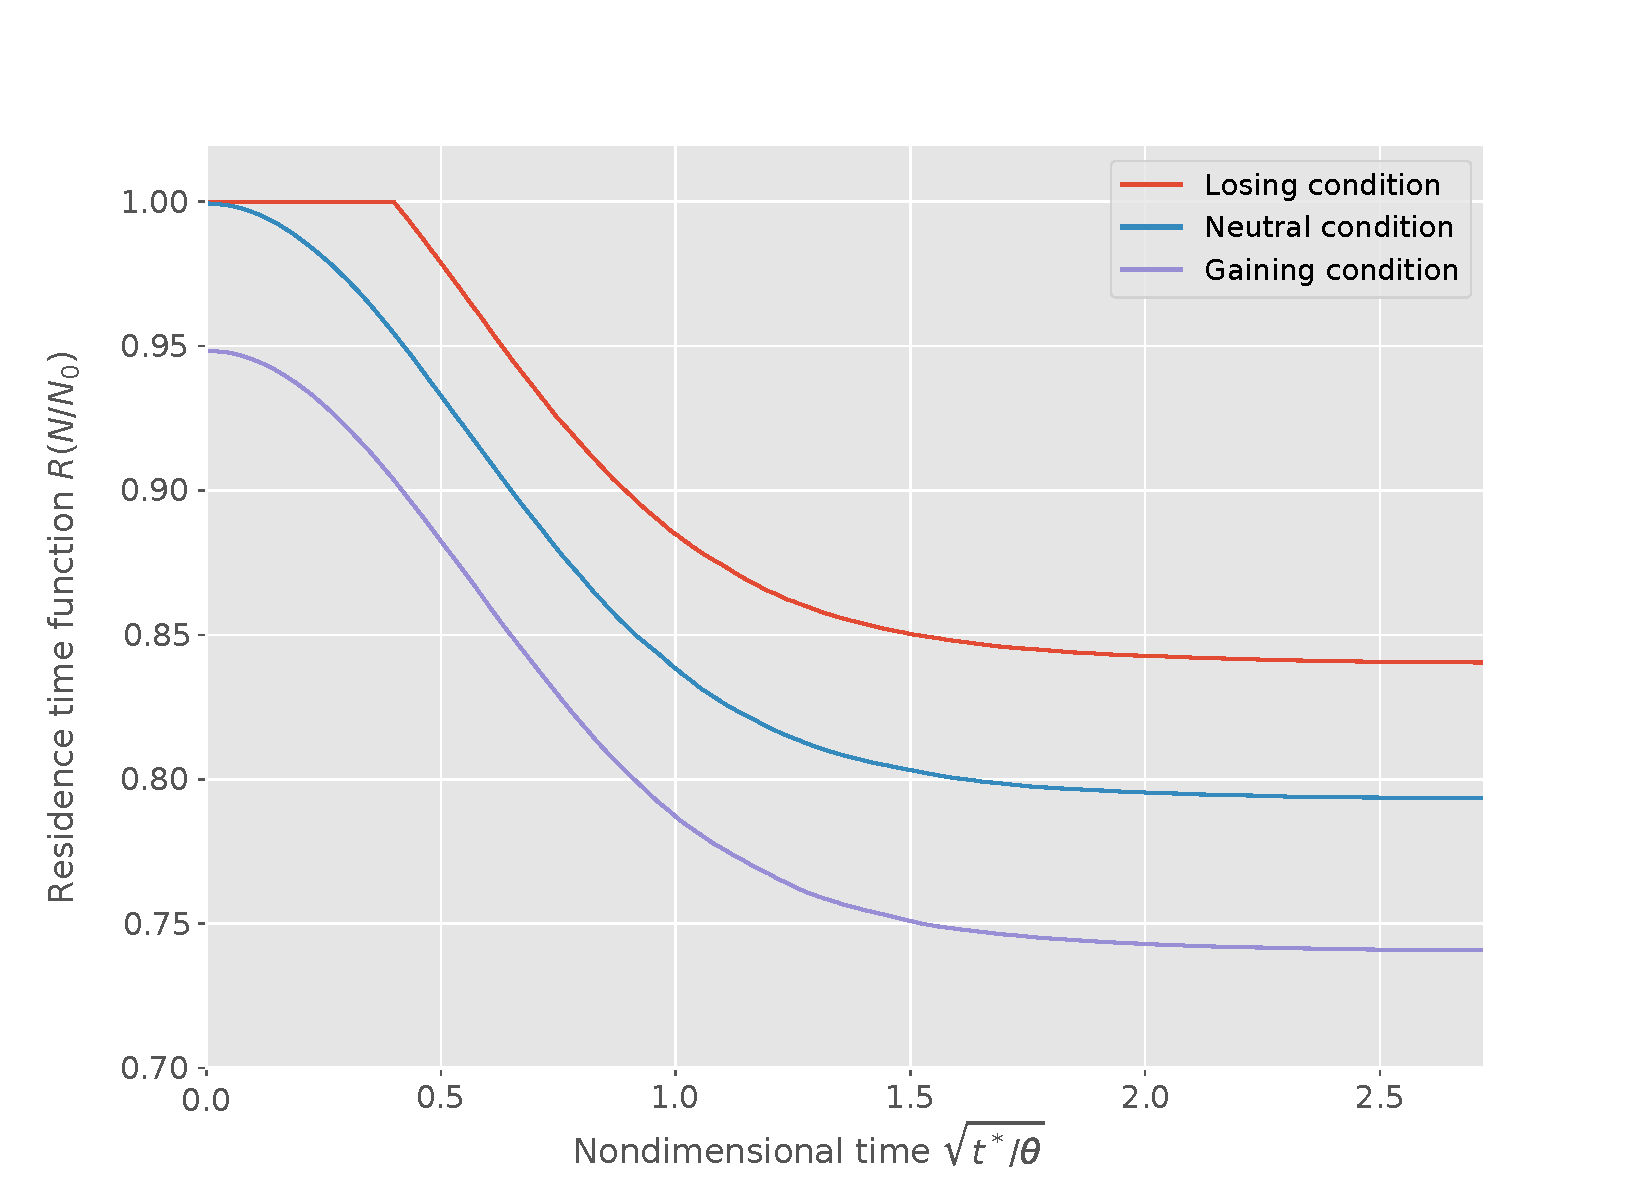
\includegraphics[trim=0.2cm 0.2cm 0.2cm 0.2cm, width=35pc]
{190131_RTF.pdf}
\caption{Residence time function for different flow conditions imposed. This plots are the Cumulative Distribution Function (CDF) of particles inside the domain in a time $\tau$ after injection.}
\label{RTF}
\end{figure}
% ============================================================================

% 5. Residence time function and the derivative (check when the other model is run)
The RTF (figure \ref{RTF}) shows that some of the particles will remain in the bed indefinitely since they have been filtered by the model and cannot be remobilized. Nevertheless, the amount of particles inside it is clearly affected by the vertical flow conditions imposed; i.e. when the losing condition is imposed particles will travel inside the domain more time and will be more likely filtered by the sand bed. In contrast, when neutral and gaining conditions are imposed, particles' streamlines will push the particles outside the domain before they are filtered. Furthermore, the RTF is not constant until late times, showing that filtration and vertical flow conditions affect fine particles' deposition.   

Although gaining and losing conditions are ``symmetrical'', the results of the RTF for the losing and gaining conditions are not equally distant from the RTF curve of the neutral condition. Moreover, this result is supported by the experimental results by \citet{Fox2018}. Actually, the losing condition RTF is closer to the neutral condition than the gaining one. To explore this, the rate of change of the RTF in time was estimated for the three cases (figure \ref{RTFder}). These curves are the Residence Time Distribution (RTD) and were obtained by taking the gradient of each RTF and then applying a convolution between the derivative and a top hat function with unit area and a span of $400$ points. 

% ============================================================================
% RTF der - figure
\begin{figure}[ht]
\centering
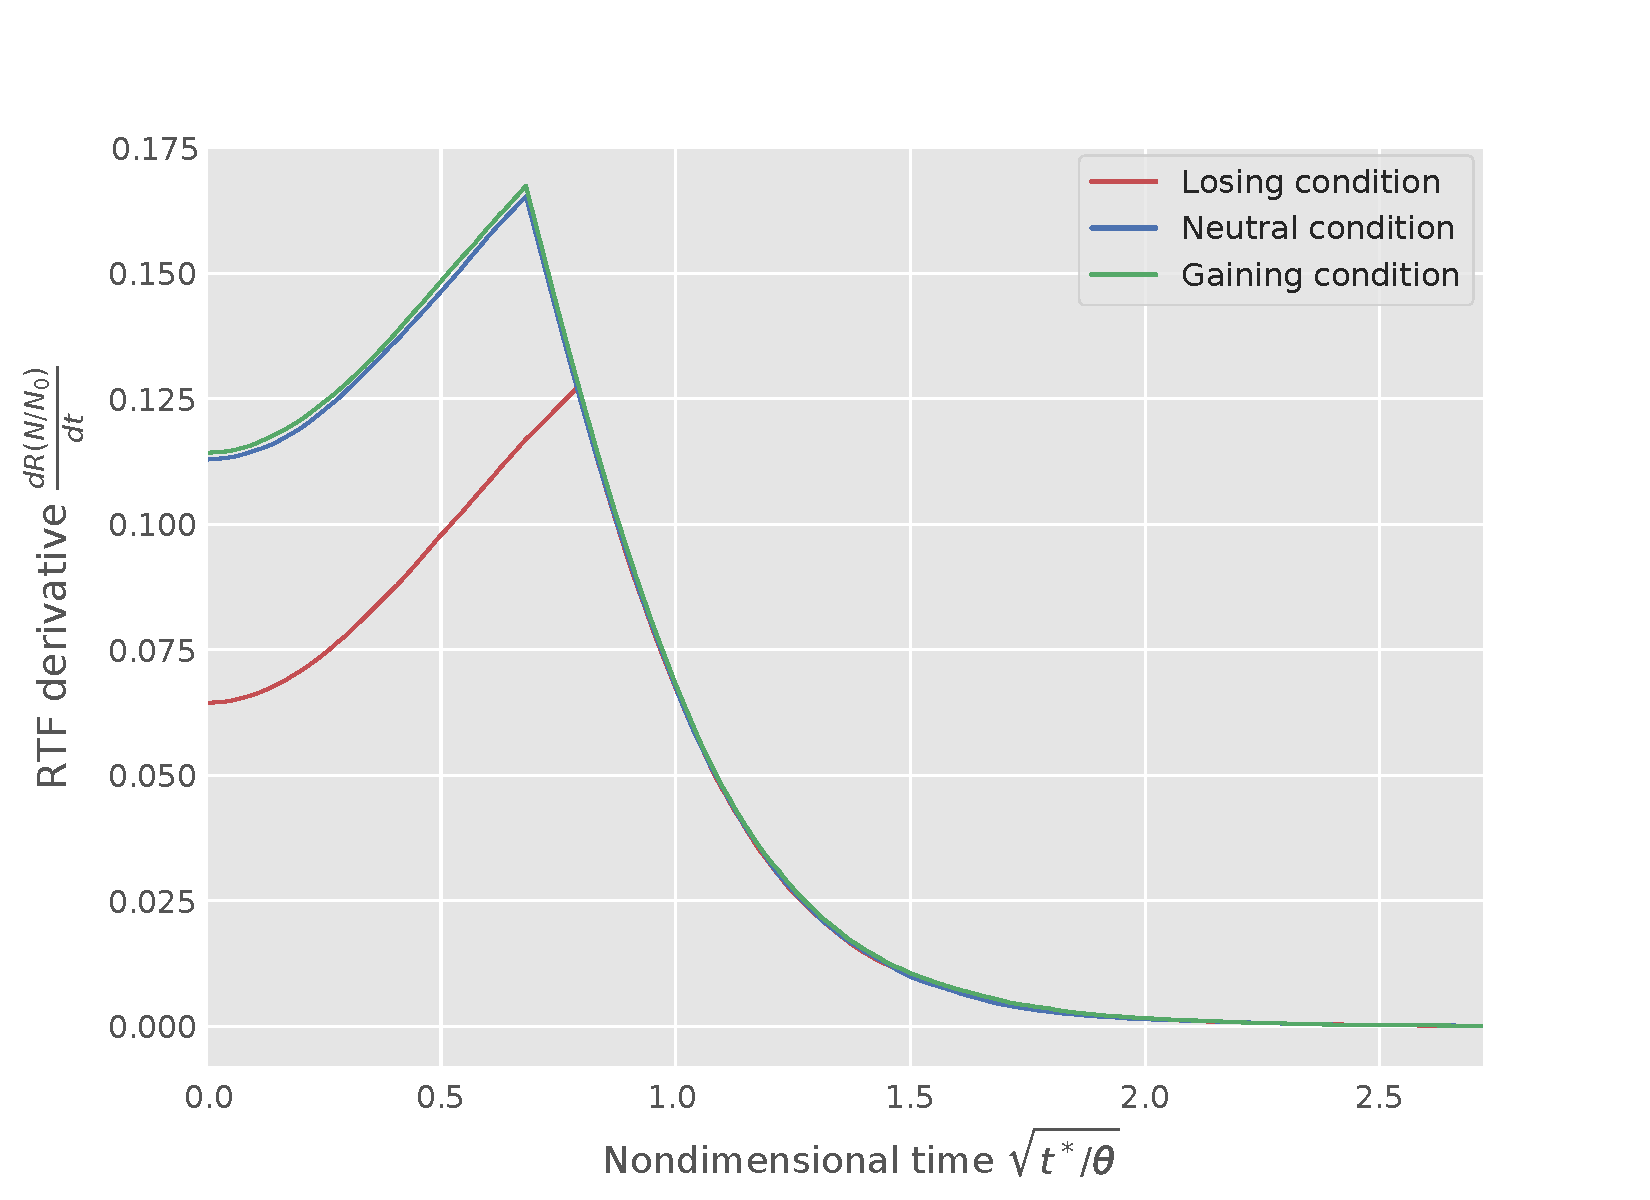
\includegraphics[trim=0.2cm 0.2cm 0.2cm 0.2cm, width=35pc]
{190131_RTF_der.pdf}
\caption{Derivative of RTF for the three vertical groundwater flow conditions modeled. This plot is interpreted as the Probability Density Function (PDF) of particles inside the domain at a given time $\tau$ after injection}
\label{RTFder}
\end{figure}
% ============================================================================

The RTF is constant at early times and starts to change after certain time that corresponds to the minimal path that a particle can travel through the domain. For the losing case, this path is longer than for the neutral and gaining cases. The RTD also reflects this feature (figure \ref{RTFder} red line), starting with a lower probability of particles leaving the domain and a maximum probability lower than in the other two conditions modeled. For the three modeled cases, the probability of a particle leaving the domain is lower at early times, then there is an increase until the peak probability of leaving the bed, and then decreasing monotonically until there are no more particles to remove.

In addition, for any time after the peak probability of leaving the domain, the rate of change of particles inside the domain is the same for the three conditions modeled (figure \ref{RTFder}). Nonetheless, in the losing condition particles are prevented to leave the domain at early times because of the longer paths of the flow condition. Yet, for neutral and gaining cases the probability of leaving the domain shown in the RTD (figure \ref{RTFder}) is higher. Indeed, the main difference between the three curves of the RTD's is shown before the peak probability of particle removal. 

% 5. COMPARISON BETWEEN NUMERICAL AND EXPERIMENTAL RESULTS FORM FOX'S PAPER
The numerical model results are compared with the experimental results from \citet{Fox2014,Fox2018}. For the physical experiments the dunes were divided in four locations, each one corresponding to a quarter part of the dune (\ref{Conceptual}c). Then, cores were extracted and the portion of clay in mass was estimated for different depths every $0.5 \ cm$ and different locations. 

Therefore, to compare experimental results with the PT model, the non-dimensional domain is divided in sections of $\pi/2$ width. Then, the mean relative number of particles is counted for every dune location and the mean and standard deviation of particles are estimated. Accordingly, the mean mass fraction of clay is compared with the mean relative number of particles in every location and the standard deviation of the experimental measurements is compared with the standard deviation of relative number of particles (figure \ref{Comparison}).  

% ============================================================================
% Comparing with experimental results - figure
\begin{sidewaysfigure}
\centering
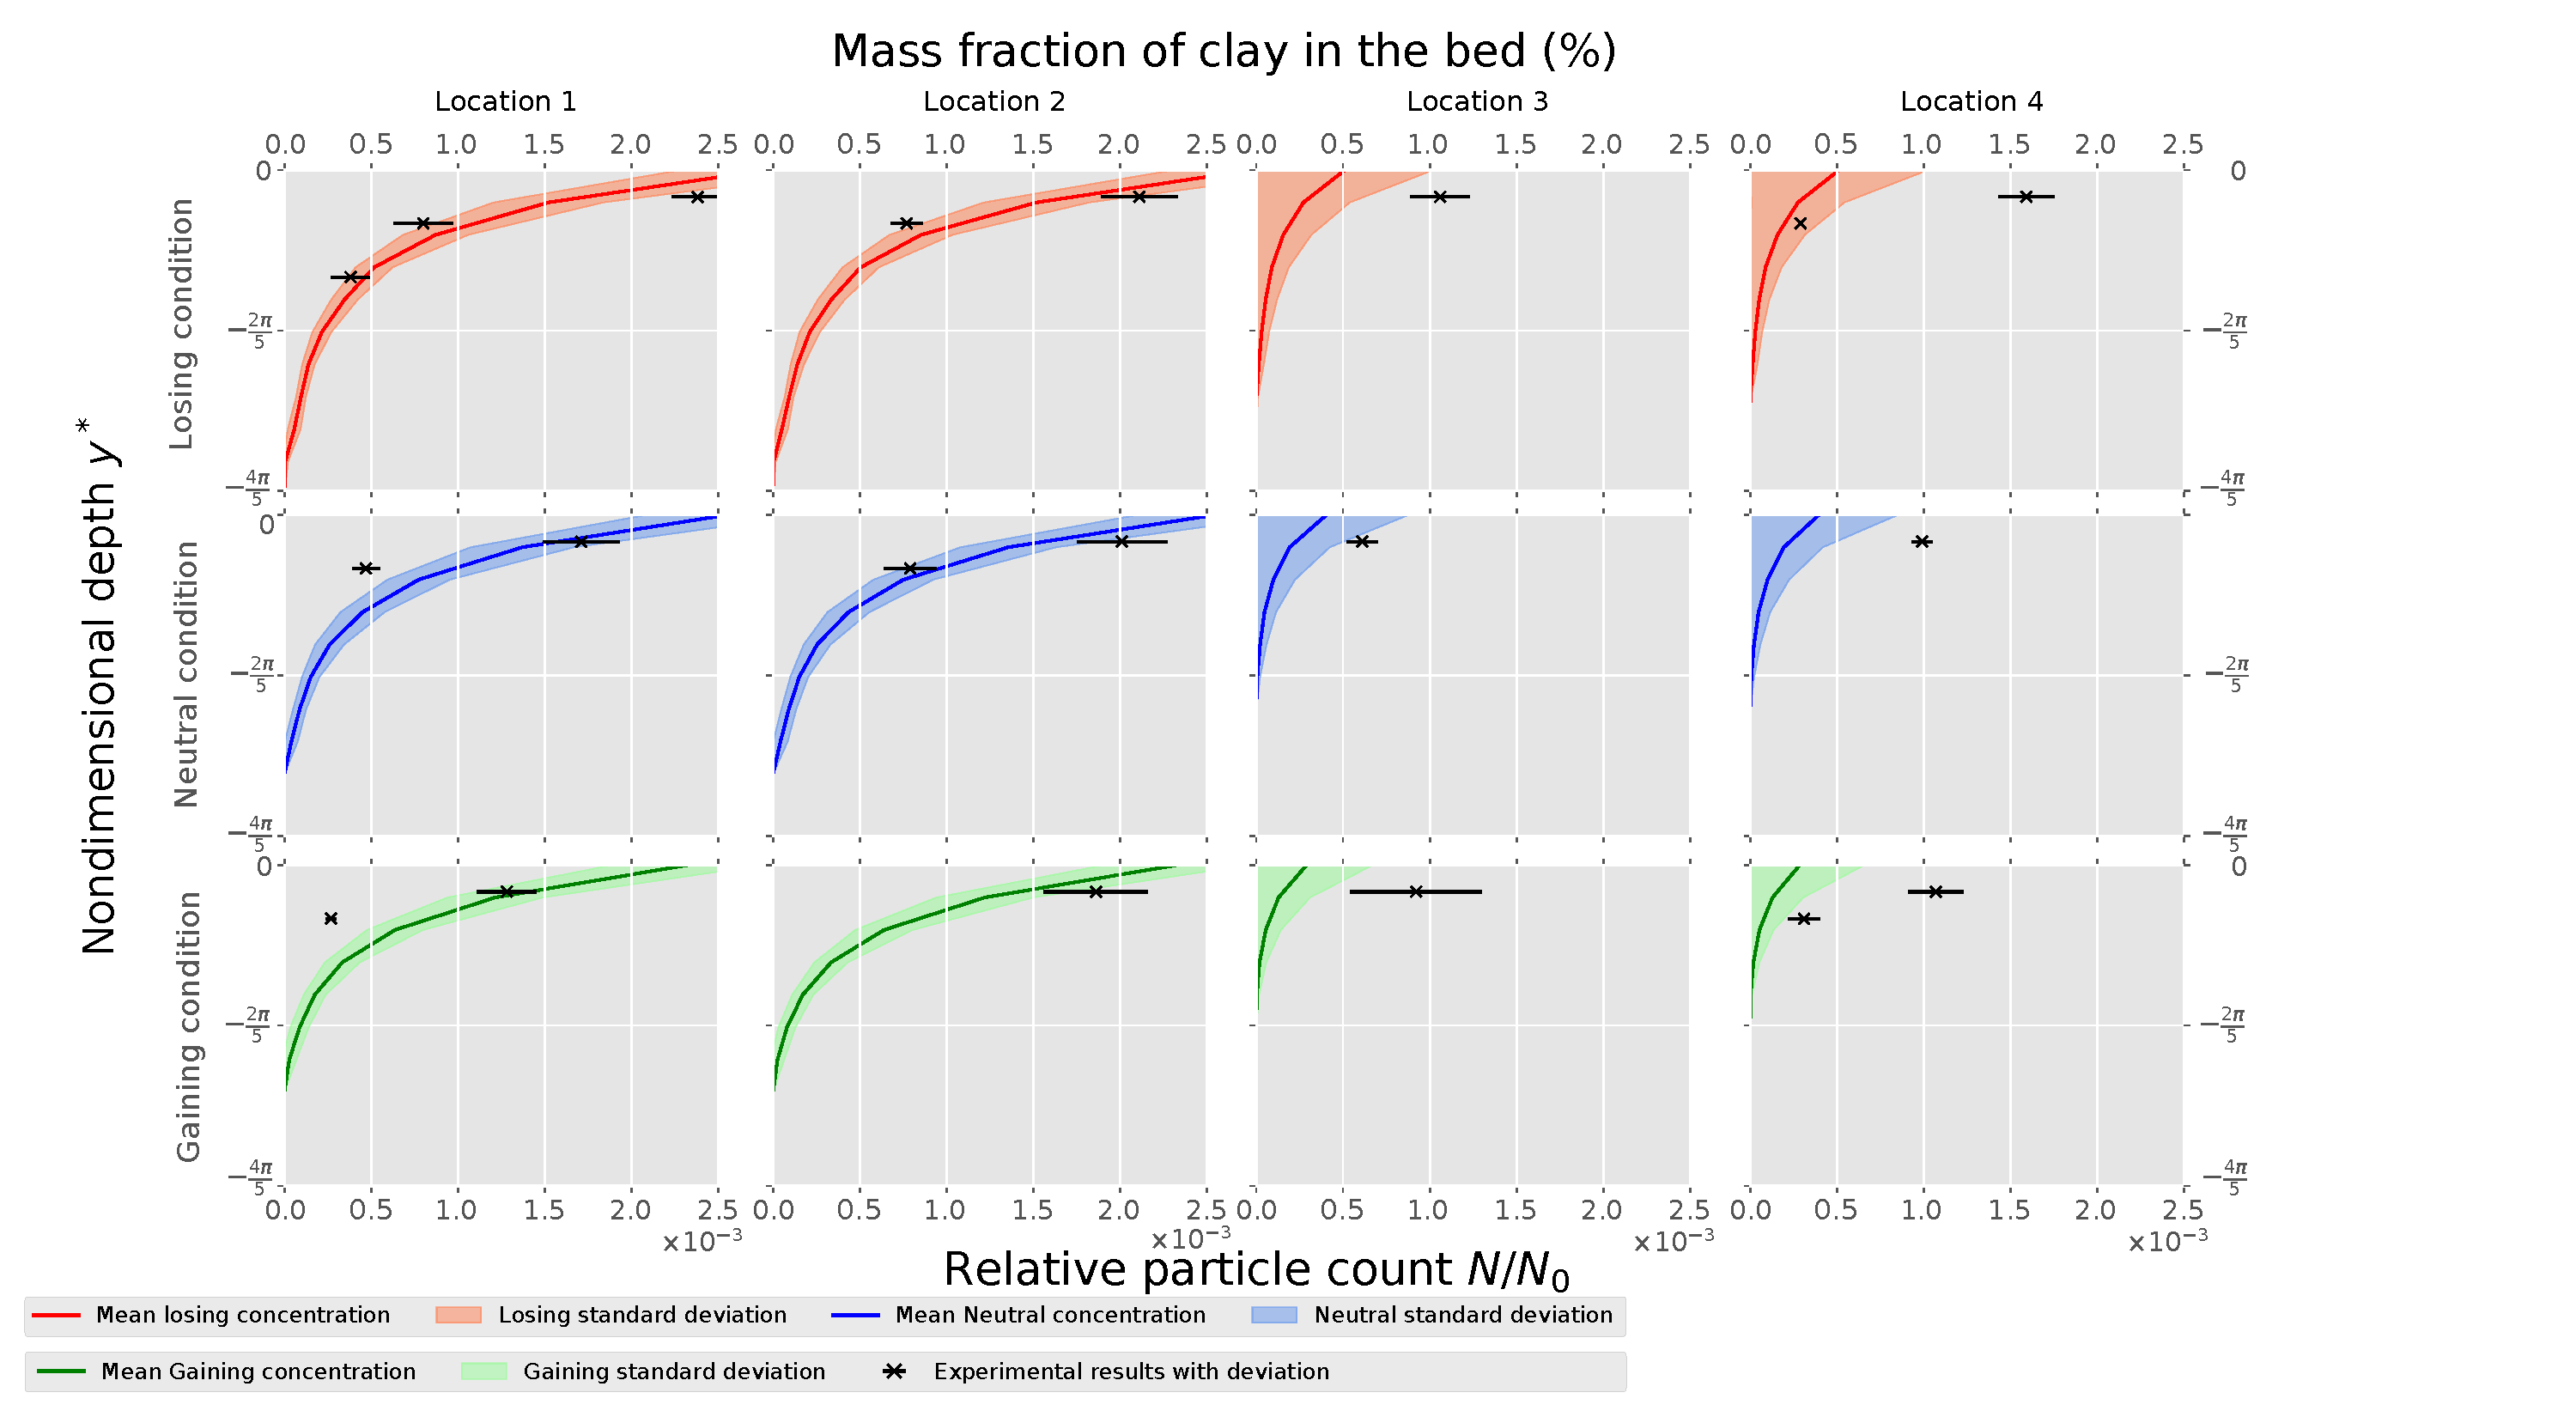
\includegraphics[trim=0.2cm 0.2cm 0.2cm 0.2cm, width=65pc]
{190131_Comparing.pdf}
\caption{Comparison with experimental results from \citep{Fox2018}. The top horizontal axis represents the fraction of clay mass found in the experiments expressed in $\%$. The bottom horizontal axis represents the fraction of particles of the numerical domain. Solid colored lines represent the average fraction of particles over depth for the different locations. Shaded areas represent the standard deviation of the fraction of particles over depth at different locations. Crosses are the mean mass fraction sampled in the experiments, and black lines represent the standar deviation of the measurements.}
\label{Comparison}
\end{sidewaysfigure}
% ============================================================================

The superposition of the experimental results and the physical experiments shows that there is a similar behavior in the decay of fine particles' concentration over depth for the three mentioned cases, particularly in locations 1 and 2 (figure \ref{Comparison}).  

Fine particles' deposition varies according to the location that is analyzed. In other words, particles tend to deposit more in locations one and two (the stoss side of the dune), and reduce their deposition in locations three and four (lee side of the dune). In fact, the deposition in the latter is provided by the particles that move from right to left in the computational domain following the path lines (figure \ref{Velocities}). In general, for the three cases modeled, more fine particles are found in the stoss side of the domain, and this phenomenon is clearly explained by the shape of the provided velocity profiles (figure \ref{Velocities}). Nevertheless, for all of the three cases modeled, the experimental results show more clay over depth for locations three and four (\ref{Comparison}), i.e. the lee side of the domain. 

Our results show strong similarities between the experimental results and the PT model, particularly in locations 1 and 2 of the sand dune (figure \ref{Comparison} first two columns). Nonetheless, there are notable differences between the numerical PT model and the experimental results in the lee side of the dune (figure \ref{Comparison} columns 3 and 4). More specifically, in the lee side of the dune, the PT model underestimates the concentration of particles when compared with experimental results, in all of the three compared conditions. However, the similarities of the PT model with the experimental results are able to highlight the contribution of filtration and vertical flow. 

% ================================================================================
% DISCUSSION SECTION
% ================================================================================
\section{Discussion} \label{Discussion}

% 1. Velocity profiles and deposition patterns analyzed
The proposed PT model departs from and ADE and combines it with a stochastic filtration framework \citep{Li2017} to simulate fine particles' deposition. Moreover, it does not pose any problems regarding mass conservation, artificial diffusion or unwanted oscillations provoked by numerical scheme instabilities \citep{Delay2005}. The results are physically consistent with experiments and also follow a mean continuum behavior expected.

Regarding the individual particle behavior, the Stokes number value for ech one is so low that it is safe to assume that they follow perfectly the streamlines. In particular, this assumption is made because of the size of a typical clay particle and the maximum velocity which it is subject to when entering the streambed that is being modeled. In fact, if the low Stokes number assumption is followed for the maximum velocity, it will hold for any lower velocity (equation \ref{STK}).

Stokes number is defined as the relation between the stopping distance and the characteristic length of the phenomenon \citep{Clark2009}. For our model, it was shown in sub subsection \ref{Mathematical_model}. Consequently, the phenomenon of settling velocity inside the sand bed is not taken into account as it was in previous works \citep{Packman2000}.

Important differences arise when comparing deposition patterns from the three conditions modeled. In fact, the gaining flow condition produces less deposition than the neutral and losing condition. However, deposition is present only at the top of the domain in all of the modeled cases, because of the velocity profiles generated by the dune shapes and the imposed vertical groundwater flow.

Furthermore, deposition patterns (figure \ref{Logmap}), show that a change in the vertical flow conditions affect not only the maximum penetration depth of the particles, but also the horizontal extent of the particles' cloud. In that sense, particles' presence in the streambed will cover more dune's width in the losing condition and it will tend to be less in the neutral and gaining cases (figure \ref{Logmap}). This explains the decay in hyporheic exchange in the experiments run with conservative tracers after clay injections under different vertical flow conditions \citep{Fox2014,Fox2018}. Namely, when fine particles cover a bigger portion of the dune wavelength, the penetration of a conservative tracer is hindered because of the fine particles' deposition. 

In addition, the PT model shows that the velocity profiles and filtration produce stratified horizontal layers. In other words, fine particles' penetration is stratified for all of the modeled cases, but these layers have different widths according to the groundwater inflow case. Therefore, our results suggest agreement with experimental results that clearly show an uneven distribution of clay mass in the dunes \citep{Fox2018}.

The decay of mean clay concentration with depth is similar to the experimental results presented by \citet{Fox2018}. However, the standard deviation of clay's mass fraction in the experiments is not similar to the PT model's results. This difference can be explained by the difference in shape of the dunes in the experiment and the proposed dune for the numerical model. For the experimental set up, the shape of the dunes and the material porosity are not homogeneous because of the normal conditions of the experiment. Nevertheless, our model simulates and idealized dune with a fixed shape and constant physical properties inside the domain.   

% 2. Discussion about the particle's behavior over time (remobiliztion, RTF and what does that imply in the context of clay deposition) [THIS PARAGRAPH NEEDS TO BE REWRITTEN EXPLAINING THE FIGURES]
The particles' behavior over time for each of the modeled case is unique, i.e. each one of the vertical flow conditions has three characteristic curves (figure \ref{Pvst}). For the losing case the maximum fraction of filtered particles by the end of the simulation is $0.82$; while it is $0.76$ and $0.76$ for the neutral and gaining cases, respectively. Regarding the fraction of particles that escaped the domain, values of $0.17$, $0.20$ and $0.24$ are reported for the losing, neutral and gaining cases, respectively. The latter results suggest that the vertical flow imposed plays a crucial role in affecting the filtering process inside the streambed. 

Furthermore, the rate of change of the RTF (figure \ref{RTFder}) suggests that the particles' movement and retention inside the domain depends also on the imposed flow conditions and not just on the filtration coefficient. The RTF curves (figure \ref{RTFder}) suggest that the filtration process is the same for all of the modeled cases and that the initial particles' escape from the domain caused by the imposed flow condition is the main driver of the phenomenon analyzed. 

Consequently, in all of the cases the main difference is set at the initial times of the simulations, when particles escape or remain in the domain according to the imposed vertical velocity. In other words, particles that do not escape the domain at early times are subject to movement or filtration, and the more particles are moving inside the domain (losing condition), the more the filtration process will act during the simulation. 

In general, our model shows that clay deposition is a phenomenon that results from the combination of the velocity inside the streambed, the vertical flow condition (losing, neutral or gaining), and the filtering properties of the material. However, this process is fostered and changed drastically when a vertical flow is imposed. 

\section{Conclusions} \label{Conclusions}

The implemented PT model is a useful tool to understand how two physical processes (i.e. bedform generated flow and filtration) control fine particles' deposition in sand beds. The flow fields generated by both, flow over a dune and vertical groundwater flow, drive the fine particles inside the sand beds and generate irregular deposition patterns. 

The observed patterns are similar to the ones reported in previous experiments. The mean concentration of particles inside the domain is similar to the fraction of mass for most of the domain simulated. However, some deviations from the experimental results were found, suggesting that even if the main physical processes were captured, the heterogeneity of the natural media or the experimental flumes plays an important role in the distribution of deposited particles in the domain. 

Moreover, the effects of turbulent flows in the internal structures of the dunes arenot taken into account in these type of models that use steady velocity fields for estimating the particles' position in every timestep. In addition, the changes in porosity (hence permeability) of the media due to the particles' deposition must have an effect in the velocity profiles. However, our model provides the basic understanding of the depositon phenomena and opens the door for further research in the topic of deposition under heterogeneous conditions. 

\acknowledgments
This research was funded by Colciencias grant 647; the James W. Fulbright Association under the program of visiting doctoral student; the HERMES mobility system of Universidad Nacional de Colombia; the US - Israel NSF-BSF grant EAR-1734300. Supporting information codes are available at (FIGSHARE\_URL). Authors declare no conflicts of interest.
The url with the codes will be provided with its DOI as with the revision of the paper. 
% References and Citations
\bibliography{Paper_PT.bib}

% % FIGURE IN THE END OF THE DOCUMENT TO MATCH DRAFT SUBMISSION

% % ============================================================================
% % Conceptual model of the problem proposed - figure
% \begin{figure}[ht]
% \centering
% \includegraphics[clip, trim=4.2cm 4.5cm 8cm 3cm, width=18pc]
% {1807010Conceptual.pdf}
% \caption{Conceptual model for the posed problem}
% \label{Conceptual}
% \end{figure}
% % ============================================================================

% % ============================================================================
% % Velocity profiles - figure
% \begin{figure}[ht]
% \centering
% \includegraphics[trim=2cm 1.5cm 4cm 0.1cm, width=25pc]
% {181203_Streamlines.pdf}
% \caption{Streamlines under different vertical flow conditions: (A) Losing, (B) Neutral and (C) Gaining. Plots' domains are shifted from $[0, 2 \pi]$ to $[-\pi /2, \pi/2]$ since domain is periodic. Note that the vertical scale is distorted.}
% \label{Velocities}
% \end{figure}
% % ============================================================================

% % ============================================================================
% % Numerical model of the problem proposed - figure
% \begin{figure}[ht]
% \centering
% \includegraphics[clip, trim=4.2cm 4.5cm 8cm 3cm, width=18pc]
% {181129Numerical.pdf}
% \caption{Depiction of numerical model proposed}
% \label{Numerical}
% \end{figure}
% % ============================================================================

% % ============================================================================
% % Concentration map - figure
% \begin{figure}[ht]
% \centering
% \includegraphics[trim=0.2cm 0.2cm 0.2cm 0.2cm, width=45pc]
% {181203_Concentrations.pdf}
% \caption{Particle deposition in different times (rows), and under different inflow/outflow conditions (columns) (Note that axis are not to scale).}
% \label{Heatmap}
% \end{figure}
% % ============================================================================

% % ============================================================================
% % Logarithm of concentration - figure
% \begin{figure}[ht]
% \centering
% \includegraphics[trim=0.2cm 0.2cm 0.2cm 0.2cm, width=45pc]
% {181203_Logplot.pdf}
% \caption{Logarithm of particle deposition in different times (rows), and under different inflow/outflow conditions (columns) (Note that axis are not to scale).}
% \label{Logmap}
% \end{figure}
% % ============================================================================

% % ============================================================================
% % Particles in time - figure
% \begin{figure}[ht]
% \centering
% \includegraphics[trim=0.2cm 0.2cm 0.2cm 0.2cm, width=35pc]
% {181203_Pvst.pdf}
% \caption{Particle's behavior over time. A. Losing condition. B. Neutral condition and C. Gaining condition}
% \label{Pvst}
% \end{figure}
% % ============================================================================

% % ============================================================================
% % Residence time function - figure
% \begin{figure}[ht]
% \centering
% \includegraphics[trim=0.2cm 0.2cm 0.2cm 0.2cm, width=20pc]
% {181203_RTF.pdf}
% \caption{Residence time function for different flow conditions imposed}
% \label{RTF}
% \end{figure}
% % ============================================================================

% % ============================================================================
% % RTF der - figure
% \begin{figure}[ht]
% \centering
% \includegraphics[trim=0.2cm 0.2cm 0.2cm 0.2cm, width=20pc]
% {181203_RTF_der.pdf}
% \caption{Derivative of RTF for the three conditions}
% \label{RTFder}
% \end{figure}
% % ============================================================================

% % ============================================================================
% % Moving der - figure
% \begin{figure}[ht]
% \centering
% \includegraphics[trim=0.2cm 0.2cm 0.2cm 0.2cm, width=20pc]
% {181203_Moving_der.pdf}
% \caption{Derivative of moving particles inside the domain}
% \label{MOVder}
% \end{figure}
% % ============================================================================

% % ============================================================================
% % Comparing with experimental results - figure
% \begin{figure}[ht]
% \centering
% \includegraphics[trim=0.2cm 0.2cm 0.2cm 0.2cm, width=40pc]
% {181203_Comparing.pdf}
% \caption{Comparison with experimental results from \citep{Fox2018}}
% \label{Comparison}
% \end{figure}
% % ============================================================================

\end{document}